\documentclass[11pt]{article}
\usepackage{psfig}
\usepackage{latexsym}
\usepackage{amsfonts}
\usepackage{amsmath}
\usepackage{mathtools}
\usepackage{tikz}
\usepackage{amsthm}


\setlength{\textheight}{8.5in}
\setlength{\textwidth}{6.0in}
\setlength{\headheight}{0in}
\addtolength{\topmargin}{-.5in}
\addtolength{\oddsidemargin}{-.5in}


\input{preamble.tex}

\begin{document}

\lecture{5}{January 25, 2018}{Arpita Patra}{Pranshu Gaba}

\section{Introduction}
Last time, we looked at computational security,  and made the definitions of probabilistic polynomial-time (\ppt)/negligible function precise in terms of security parameter \(n\). We looked at the semantic and the indistinguishability based definitions of security and showed that they are equivalent. We also looked at pseudorandomness and pseudorandom generators (PRGs).

Now we will continue the discussion on PRGs. We will make use of reduction-based proofs to prove that if PRGs exist, then a construction is secure according to ind-secure definition. We will find a construction for COA-secure symmetric key encryption, and finally, discuss the short comings of the current construction/definition, and try to come up with a better 1definition.  

\section{Pseudorandom Generators (PRGs) \cite{katz} \cite{patra}}

Let \(l(n)\) be a polynomial such that \(l(n) > n\) for all \(n\). Let \(U\) be the uniform distribution over \(\{0, 1 \} ^{l(n)}\). Let \(G \colon \{0, 1\}^n \to \{0, 1\}^{l(n)}\) be a length-expanding function with probability distribution over \(\{G(s) : s \in _{R} \{0, 1\}^n \}\).

To determine whether \(G\) is a PRG, a game is played. A \ppt\ distinguisher \(D\) asks the challenger for a string of length \(l(n)\). The challenger flips a coin \(b\). If \(b = 0\), then the challenger picks a string from \(U\). If \(b = 1\), then the challenger picks a string from \(G\). The distinguisher must now tell if the string was chosen from \(U\) or \(G\). If the distinguisher guesses correctly, then we say \(D(y) = 1\), else \(D(y) = 0\).

We say that \(G\) is a PRG if for every \ppt\ distinguisher \(D\), there is a negligible function \negl\ such that
\[ \big| \underset{r \in _R \{0, 1\}^{l(n)}}{\mathrm{Pr}[D(r) = 1]} - \underset{s \in _R \{0, 1\}^n}{\mathrm{Pr} [D(G(s)) = 1]} \big| \le \mathsf{negl}(n) \]

That is, the difference in probabilities of the adversary winning the game when the number is chosen from \(U\), and when the number is chosen from \(G\), should be negligible.

\subsection{Attempt to construct a PRG}
We will now try to construct a PRG. We have \(s \in _R \{0,1\}^n\).  Consider the function \(G \colon \{0, 1\}^n \to \{0, 1\}^{n+1}\), which is defined to be  \(G(s) = ss'\), where \(s' = \Xor _{i = 1}^n s_i = s_1 \xor s_2 \xor \cdots \xor s_n\). Note that output of \(G\) is one bit longer than \(s\), so expansion factor \(l(n)\) is \(n + 1\). 

Given a string from \(y \in \{0, 1\}^{n+1}\), the distinguisher must determine if it is generated from \(U\) or \(G\), i.e. the distinguisher tries to guess the value of \(b\).  

The strategy adopted by a efficient distinguisher \(D\) is to output 1 if and only if the last bit of the message is equal to the XOR of all the preceding bits. There are two possible cases:
\begin{itemize}
    \item If the last bit does not equal the XOR of all the preceding bits, the distinguisher \(D\) knows for sure that the message was from \(U\). He guesses \(b\) correctly. \(\mathrm{Pr}[D(r) = 1] = 1\)
\item Else if the last bit equals the XOR of all preceding bits, then there are two possible cases again:
\begin{itemize}
    \item If \(y\) is from \(G\), then \(D\) is always correct.
    \(\mathrm{Pr}[D(G(s)) = 1] = 1\), \( s \in _R \{0, 1\}^n\).
    \item Else if \(y\) is from \(U\), then \(D\) is correct with half probability. \(\mathrm{Pr}[D(r)] = 1] = \frac{1}{2}\), \(r \in_R \{0, 1\}^{n+1}\).
\end{itemize}
\end{itemize}

The difference in the probabilities is 
\[\big| \mathrm{Pr}[D(r) = 1] - \mathrm{Pr}[D(G(s))] = 1] \big| = 1 - \frac{1}{2}\]
This difference is constant, and not negligible, thus \(G\) that we chose is not a PRG. As it turns out, constructing a PRG is a very difficult task.

\subsection{PRG can be cracked by an unbounded adversary}
Consider the length-doubling PRG, where \(G\) takes in a seed of length \(n\), and outputs a string of length \(2n\). There are \(2^n\) possible strings of length \(n\), and \(2^{2n}\) strings of length \(2n\). If an adversary picks a  string from \(\{0, 1\}^{2n}\) uniformly at random, then the probability that he picks a strings that came from a seed is \(\frac{2^n}{2^{2n}} = \frac{1}{2^n}\), which is negligible.  Most of the \(2n\) length strings do not appear as the output of \(G\). There is a negligible probability that he picks a string from the range of \(G\). 

If a \ppt\ adversary is given a string \(y\), then there is negligible probability that he will be able to distinguish correctly whether it is from \(U\) or \(G\). This is because he cannot compare \(y\) with all the \(2^n\) outputs of \(G(s)\) in polynomial time. 

However, if we give the adversary unbounded power, then he can list out all those \(2^n\) outputs of \(G(s)\). Then given any string \(y\), he can check if it belongs in the range of \(G\). The adversary's strategy would be:

\begin{itemize}
    \item If \(y\) is in not the range of \(G\), the distinguisher outputs \(0\) always because it was definitely not generated by \(G\). 
    \item Else if \(y\) is in the range of \(G\), then the optimal strategy of \(D\) is to output 1 always. 
    \begin{itemize} 
    \item If \(y\) is from \(G\), then \(D\) is always correct. \(\mathrm{Pr}[D(G(s)) = 1] = 1\), \( s \in _R \{0, 1\}^n\).
    \item Else if \(y\) is from \(U\), then \(D\) is correct with probability \(\frac{2^n}{2^{2n}}\).  \(\mathrm{Pr}[D(r) = 1] = 2^{-n}\), \(r \in_R \{0, 1\}^{n+1}\).

    \end{itemize}
\end{itemize}

When we test the security of this scheme, we see that the distinguisher is almost always able to distinguish correctly. 
\[ \big| \mathrm{Pr}[D(r) = 1] - \mathrm{Pr}[D(G(s)) = 1] \big| \ge \underbrace{1 - 2^{-n}}_\textrm{not negligible}\]
The difference in probabilities is \(1 - 2^{-n}\), which is not negligible, so this scheme can be cracked by an unbounded adversary. 

Cryptography is an applied science, and in reality, the adversary does not have unbounded power. It is reasonable to construct a scheme that can be broken by a \ppt\ adversary only with at most negligible probability. However, while implementing this algorithm, it must be made sure that \(n\) is large enough so it cannot be broken using brute-force by a \ppt\ adversary in a reasonable time.

In this entire section, we have assumed that PRGs exist. Their existence has neither been proven nor disproven, although it is strongly believed that they exist. However, it has been shown that if one-way functions exist (which are a lower-level primitives than PRGs), then PRGs exist \cite{goldreich}. We also believe that stream ciphers are PRGs, because no good distinguishers for them are known.



\subsection{One-way functions}
One-way functions are functions that are easy to compute, but almost always difficult to invert. We can play a game \(\mathsf{Invert}_{\mathcal{A},f} (n)\) to check if \(f\) is a one-way function. 

\subsubsection{Inverting game}

The challenger chooses number a number \(x\) from \(\{0, 1\}^n\) uniformly at random, and computes \(y \coloneqq f(x)\). A \ppt\ adversary \(\mathcal{A}\) is given \(y\). The adversary now tries to guess \(x'\), a pre-image of \(y\).

If \(f(x') = y\), then the adversary has won, and the output of the game is 1.
Else if \(f(x') \neq y\), then the adversary has lost, and the output of the game is 0. Note that \(\mathcal{A}\) does not have to find the original \(x\) to win the game. It is sufficient for him to guess any pre-image to win the game. 

We say that \(f\) is one-way if \(\mathcal{A}\) wins the game with negligible probability.

\subsubsection{Mathematical formulation}
Function \(f \colon \{0, 1\}^* \to \{0, 1\}^*\) is a {\sf one-way function}  if the following two conditions hold:
\begin{itemize}
\item Easy to compute: for every \(x \in \{0, 1\}^*\), \(f(x)\) can be computed in \poly \((n)\) time.
\item Hard to invert: For every \ppt\ algorithm \(A\), there is a negligible function \negl\((n)\) such that
  \[ \mathrm{Pr}[\mathsf{Invert}_{\mathcal{A}, f} (n) = 1] \le \mathsf{negl}(n) \approx \mathrm{Pr} _{x \leftarrow \{ 0, 1\}^n} [\mathcal{A}(f(x), 1^n) \in f^{-1} (f(x))] \le \mathsf{negl}(n) \]
\end{itemize}


\section{Proofs by Reduction}
Proofs by reduction are very useful. We can use them to prove statements like
\begin{enumerate}
    \item If an encryption scheme \(\Pi\) is secure, then another scheme \(\Pi'\) is also secure. 
    \item If an assumption \(A\) holds, then \(\Pi\) is secure. 
    \item If \(A_1\) holds, then \(A_2\) also holds.
    \item If \(\Pi\) is secure, then \(A\) holds.
\end{enumerate}

Proof by reduction involves proof by contradiction/contrapositive. We will see how to prove statement 1. The other statements can be proved in a similar fashion. 

We want to prove that if \(\Pi\) is secure, then \(\Pi'\) is also secure. 

\begin{prooof}
    Assume that \(\Pi'\) is not secure, so we have a \ppt\ attacker against \(\Pi'\) that can break it with non-negligible probability \(f(n)\). The challenger sends a challenge for \(\Pi\) to \ppt\ attacker against \(\Pi\).  Based on this challenge, the \ppt\ attacker against \(\Pi\) sends a simulated challenge to \ppt\ attacker against \(\Pi'\). This \ppt\ can break \(\Pi'\) with non-negligible probability \(f(n)\). 
    
    Based on this break, the \ppt\ against \(\Pi\) comes up with a solution for \(\Pi\) which can break \(\Pi\) with probability \(1/p(n)\). The overall probability that the \ppt\ attacker against \(\Pi\) breaks the scheme is at least \(f(n)/p(n)\), which is not negligible. However, our statement included the assumption that \(\Pi\) is secure, so this should not be possible. This is a contradiction! Therefore \(\Pi'\) is secure, and no \ppt\ attacker against \(\Pi'\) exists that can break with probability \(f(n)\).

    \noindent
    \begin{tikzpicture}
        \path (0,0) rectangle (15, 2.3);
        \node at (0.75,1) {\includegraphics[width=2cm]{shenyong6345_014}};
        \draw [->] (2,1.35) -- (6,1.35);
        \node at (4,1.62) {A challenge for \(\Pi\)};
        \draw [<-] (2,0.25) -- (6, 0.25);
        \node at (0.75,-0.3) [align=center, text width = 2cm]{Challenger };
        \node at (4,0.25) [align=center, text width = 5cm]{Solution with \\ probability \(1/p(n)\)};
        \node at (7.25,1) {\includegraphics[width=2cm]{attacker}};
        \node at (7.25,-0.42) [align=center, text width = 2.5cm]{\ppt\ attacker \\ against \(\Pi\) };
        \draw [->] (8.5,1.35) -- (12.5,1.35);
        \draw [<-] (8.5,0.3) -- (12.5, 0.3);
        \node [align=center, text width = 5cm] at (10.5,1.35) {Simulation of a\\ challenge for \(\Pi'\)};
        \node [align=center, text width = 5cm] at (10.5,0.3) {Break with\\ probability \(f(n)\)};
        \node at (13.75,1) {\includegraphics[width=1.45cm]{duivel}};
        \node at (13.75,-0.42) [align=center, text width = 2.5cm]{\ppt\ attacker \\ against \(\Pi'\)  };
    \end{tikzpicture}
\end{prooof}


\section{COA-secure SKE}
%%%% TODO: Check for errors
We now construct a scheme \(\Pi\) that is COA-secure using the ind-secure definition. That is, for every \ppt\ adversary \(\mathcal{A}\), there is a negligible function \negl, such that 
\[\mathrm{Pr}\big[\mathsf{PrivK}^{\mathsf{coa}}_{\mathcal{A}, \Pi} (n)= 1\big] \le \frac{1}{2} + \mathsf{negl}(n)\]

Let \(\mathcal{K} = \{0,1\}^n\), and \(\mathcal{M}  = \mathcal{C} = \{0,1\}^{l(n)}\).

The {\sf Gen} algorithm picks a key \(k \in _R \mathcal{K}\) uniformly at random. 

The {\sf Enc} algorithm receives a key \(k \in \mathcal{K}\), and a message \(m \in \mathcal{M}\) and outputs the ciphertext \(c \coloneqq G(k) \xor m\). 

The {\sf Dec} algorithm receives a key \(k \in \mathcal{K}\) and a ciphertext \(c \in \mathcal{C}\) and outputs the message \(m \coloneqq G(k) \xor c\).

Look at \(\mathsf{Dec}_k ( \mathsf{Enc}_k(m))\). It is equal to \(m\) for all \(m \in \mathcal{M}\), since \(G(k) \xor G(k) \xor m = m\). This proves the correctness of this scheme. Using proof by reduction, we will show that if \(G\) is a PRG, then the above scheme is COA-secure.




\begin{prooof} We prove by contradiction. If \(\Pi\) is not secure, then we show that it implies \(G\) is not a PRG, which is a contradiction, so \(\Pi\) must be secure. 

If \(\Pi\) is COA-secure, then for every \ppt\ adversary \(\mathcal{A}_i\), there is a \(\mathsf{negl}_i(n)\) such that 
\begin{equation*}
\begin{split}
    \mathrm{Pr}\big[\mathsf{PrivK}^{\mathsf{coa}}_{\mathcal{A}_i, \Pi} (n) = 1\big] & \le \frac{1}{2} + \mathsf{negl}_i(n) \\ 
    & < \frac{1}{2} + \frac{1}{\poly(n)} \textrm{ for all } n > N \textrm{ for every } \poly(n)
    \end{split}
\end{equation*}

So \(\Pi\) is not COA-secure if there exists a \ppt\ adversary \(\mathcal{A}_i\) and a polynomial \(\poly_i(n)\) such that 
\[\mathrm{Pr}\big[\mathsf{PrivK}^{\mathsf{coa}}_{\mathcal{A}_i, \Pi} (n)= 1\big] > \frac{1}{2} + \frac{1}{\poly_i(n)} \textrm{ for infinitely many } n\textrm{'s}\]

Assume that \(\Pi\) is not secure. Then there exists a \ppt\ adversary \(\mathcal{A}\) such that the above inequality holds true for infinitely many \(n\)'s.

    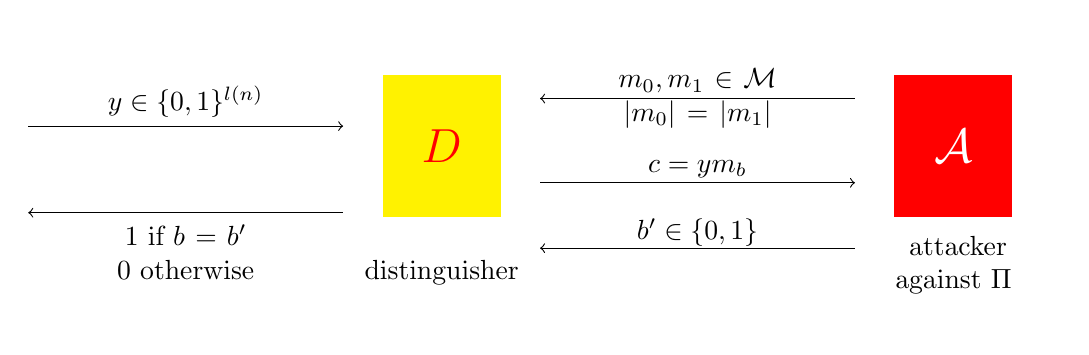
\begin{tikzpicture}
        \path (2,-1.2) rectangle (15, 2.6);
        \draw [->] (2,1.35) -- (6,1.35);
        \node at (4,1.66) {\(y \in \{0, 1\}^{l(n)}\)};
        \draw [<-] (2,0.25) -- (6, 0.25);
        \node at (4,-0.25) [align=center, text width = 2cm]{1 if \(b = b'\) \\ 0 otherwise};
        \path [fill=yellow] (6.5, 0.2) rectangle (8, 2);
        \node [color=red] at (7.25, 1.1) {\LARGE \(D\)};
        \node at (7.25,-0.42) [align=center, text width = 2.5cm]{\ppt\ \\ distinguisher };
        \draw [<-] (8.5, 1.7) -- (12.5, 1.7);
        \draw [->] (8.5,0.63) -- (12.5,0.63);        
        \draw [<-] (8.5,-0.2) -- (12.5, -0.2);
        \node [align=center, text width = 2.5cm] at (10.5,1.7) {\(m_0, m_1 \in \mathcal{M}\)\\ \(|m_0| = |m_1|\)};
        \node [align=center] at (10.5,0.8) {\(c = y \xor m_b\)};
        \node [align=center] at (10.5,0) {\(b' \in \{0, 1\}\)};
        \node at (13.75,-0.42) [align=center, text width = 2.5cm]{\ppt\ attacker \\ against \(\Pi\)  };
                \path [fill=red] (13, 0.2) rectangle (14.5, 2);
        \node [color=white] at (13.75, 1.1) {\LARGE \(\mathcal{A}\)};
    \end{tikzpicture}
    
    
    The distinguisher \(D\) gets a string of length \(l(n)\) from a challenger. He uses adversary \(\mathcal{A}\) to  help him determine whether \(y\) is a random string, or a pseudorandom string. So, \(D\) plays \(\mathsf{PrivK}^{\mathsf{coa}} _{\mathcal{A}, \Pi}\) with \(\mathcal{A}\) with \(D\) as the challenger. 
    
    \(\mathcal{A}\) sends two messages, \(m_0, m_1\), of his choice to \(D\). \(D\) must use \(y\) in the challenge to get more information about \(y\) from \(\mathcal{A}\). \(D\) can do this by flipping a coin \(b\). He sends the ciphertext \(c = y \xor m_b\) to \(\mathcal{A}\). The adversary  return his guess \(b'\) to \(D\).
    
    If \(y\) is a random string, then this case is similar to a perfect security. Even if the adversary has unbounded power, he cannot guess the bit with probability more than half. \(\mathrm{Pr}[D(y) = 1] = \frac{1}{2}\)
    
    If \(y\) is a pseudorandom string, then since \(\mathcal{A}\) is a very good adversary, he can break it with non-negligible probability. \(\mathrm{Pr}[D(G(s)) = 1] > \frac{1}{2} + \frac{1}{\poly(n)}\)
    
    The difference in probabilities is not negligible.    
    \[ \big| \mathrm{Pr}[D(y) = 1] - \mathrm{Pr}[D(G(s)) = 1] \big| > \underbrace{\frac{1}{\poly(n)}}_\textrm{not negligible}\]

This means that \(G\) is not a PRG. However, since we believe \(G\) is a PRG, therefore we also believe that \(\Pi\) is a COA-secure scheme.
\end{prooof}

\section{Multiple-message COA Security}
We have the overcome one of the limitations of perfect security: the key size can now be smaller than the message size, and the scheme will still be COA-secure. However, we still can't reuse the key. We can show that if a \ppt\  adversary is allowed to play \(\mathsf{PrivK}^{\mathsf{coa}}_{\mathcal{A}, \Pi}\) twice with the same key, then he can break  the scheme with probability 1. 


Let us define a new game, 

\[\mathsf{PrivK}^{\mathsf{coa-mult}}_{\mathcal{A}_i, \Pi} (n), \qquad  \Pi = (\mathsf{Gen}, \mathsf{Enc}, \mathsf{Dec}), \mathcal{M}.\]

This is very similar to \(\mathsf{PrivK}^{\mathsf{coa}} _{\mathcal{A}, \Pi}\), the only difference being that the adversary sends two vectors of his choice, \(\vec{M_0} = (m_{0,1}, m_{0,2}, \ldots,  m_{0,t})\) and \(\vec{M_1} = (m_{1,1}, m_{1,2}, \ldots,  m_{1,t})\) instead of messages \(m_0\) and \(m_1\). Each vector has polynomially many messages.  

A scheme \(\Pi\) is COA-mult secure if for every \ppt\ adversary \(\mathcal{A}\),
the probability that \(\mathcal{A}\) wins the above game is at most negligibly better than \(\frac{1}{2}\). 

\[  \mathrm{Pr} \big[ \mathsf{PrivK}^{\mathsf{coa-mult}}_{\mathcal{A}_i, \Pi} (n)  =  1  \big] \le \frac{1}{2}+ \negl(n)\]

The game \(\mathsf{PrivK}^{\mathsf{coa}}_{\mathcal{A}_i, \Pi}\) is special case of \(\mathsf{PrivK}^{\mathsf{coa-mult}}_{\mathcal{A}_i, \Pi}\), with \(|M_0| = |M_1| = 1\). Thus if a scheme \(\Pi\) is COA-mult-secure, then it is also COA-secure. However the converse is not true. We can show that multiple-message security is stronger than single-message security  i.e. there exists a scheme which is COA-secure, but not COA-mult-secure.

The adversary can send the following two vectors \(M_0 = (\texttt{hello}, \texttt{hello})\) and \(M_1 = (\texttt{hello}, \texttt{world})\). The challenger gets a key \(k\), and flips a coin \(b\). 
\begin{itemize}
    \item If \(b = 0\), he returns \(c_1 \coloneqq\texttt{hello} \xor k, c_2 \coloneqq \texttt{hello} \xor k\).
    \item If \(b = 1\), he returns \(c_1 \coloneqq \texttt{hello} \xor k, c_2 \coloneqq \texttt{world} \xor k\).
\end{itemize}

It is now very easy, even for a \ppt\ adversary to find \(b\). He returns \(b' = 0\) if \(c_1 = c_2\) and \(b' = 1\) if \(c_1 = c_2\). He wins the game with probability 1. 
\[  \mathrm{Pr} \big[ \mathsf{PrivK}^{\mathsf{coa-mult}}_{\mathcal{A}_i, \Pi} (n)  =  1  \big] = 1\]

We have found a scheme which is COA-secure, but not COA-mult-secure. This happens because the {\sf Enc} algorithm used was deterministic. Encrypting the same message \(m\) twice with the same key twice gives the same cipher text. 
\begin{theorem*}
    If \(\Pi\) is a cipher whose {\sf Enc} algorithm is a deterministic function of the key and plaintext, then \(\Pi\) cannot have indistinguishable multiple encryptions in the presence of an eavesdropper.
\end{theorem*}

To overcome this, we must make use of a randomized encryption scheme. This solve the problem of key reuse. The same key can then be used multiple times and the scheme will still be secure.  

Next time, we will give more power to the adversary. (chosen plaintext attacks (CPA), which is stronger than both COA and COA-mult). We will construct a scheme which is CPA-secure.


\begin{thebibliography}{9}

\bibitem{katz}
  Jonathan Katz, Yehuda Lindell,
  \emph{Introduction to Modern Cryptography},
  CRC Press,
  2nd edition,
  2015.
  
  \bibitem{patra}
  Arpita Patra,  
  \emph{Cryptography}, lecture notes, Cryptography E0 235,
  Indian Institute of Science, 2018.
  
  \bibitem{goldreich}
  O. Goldreich and L. A. Levin. A hard-core predicate for all one-way functions. In
\emph{STOC ’89: Proceedings of the twenty-first annual ACM symposium on Theory of
computing}, pages 25--32, New York, NY, USA, 1989. ACM Press.
\end{thebibliography}




\end{document}
